% !TEX TS-program = xelatex
% !TEX encoding = UTF-8

% Header {{{1

% This is a simple template for a XeLaTeX document using the "article" class,
% with the fontspec package to easily select fonts.

%\documentclass[11pt]{article} % use larger type; default would be 10pt
\documentclass[12pt]{article}

\usepackage{fontspec} % Font selection for XeLaTeX; see fontspec.pdf for documentation
\defaultfontfeatures{Mapping=tex-text} % to support TeX conventions like ``---''
\usepackage{xunicode} % Unicode support for LaTeX character names (accents, European chars, etc)
\usepackage{xltxtra} % Extra customizations for XeLaTeX

%\setmainfont{Charis SIL} % set the main body font (\textrm), assumes Charis SIL is installed
%\setsansfont{Deja Vu Sans}
%\setmonofont{Deja Vu Mono}

% other LaTeX packages.....
\usepackage{geometry} % See geometry.pdf to learn the layout options. There are lots.
\geometry{a4paper, left=25mm, right=25mm, top=25mm, bottom=25mm} % or letterpaper (US) or a5paper or....
\usepackage[parfill]{parskip} % Activate to begin paragraphs with an empty line rather than an indent

\usepackage{graphicx} % support the \includegraphics command and options
\usepackage{subcaption}

\usepackage{amsmath}
\usepackage{amssymb}

\usepackage{algorithm}
\usepackage{algpseudocode}

\usepackage{listings}
\lstset{basicstyle=\ttfamily,columns=fullflexible,keepspaces=true}

%%%%%%%%%%%%%%%%%%%%%%%%%%%%%%%%%%%%%%%%%%%%%%%%%%

\title{Report 1: OpenMP}
\author{Dinh Ngoc Tu}

\begin{document}
\maketitle

%%%%%%%%%%%%%%%%%%%%%%%%%%%%%%%%%%%%%%%%%%%%%%%%%%

\section{Conversion to OpenMP}

To implement parallelization with OpenMP, all we need is to parallelize the for loop:

\begin{lstlisting}[breaklines]
void Labwork::labwork1_OpenMP() {
    int pixelCount = inputImage->width * inputImage->height;
    outputImage = static_cast<char *>(malloc(pixelCount * 3));
#pragma omp parallel for
    for (int j = 0; j < 100; j++) {     // let's do it 100 times, otherwise it's too fast!
        for (int i = 0; i < pixelCount; i++) {
            outputImage[i * 3] = (char) (((int) inputImage->buffer[i * 3] + (int) inputImage->buffer[i * 3 + 1] +
                                            (int) inputImage->buffer[i * 3 + 2]) / 3);
            outputImage[i * 3 + 1] = outputImage[i * 3];
            outputImage[i * 3 + 2] = outputImage[i * 3];
        }
    }
}
\end{lstlisting}

Additionally, we add timing code to measure OpenMP performance:

\begin{lstlisting}[breaklines]
labwork.labwork1_CPU();
labwork.saveOutputImage("labwork2-cpu-out.jpg");
printf("labwork 1 CPU elapsed %.1fms\n", lwNum, timer.getElapsedTimeInMilliSec());
timer.start();
labwork.labwork1_OpenMP();
labwork.saveOutputImage("labwork2-openmp-out.jpg");
printf("labwork 1 OpenMP elapsed %.1fms\n", lwNum, timer.getElapsedTimeInMilliSec());
\end{lstlisting}

%%%%%%%%%%%%%%%%%%%%%%%%%%%%%%%%%%%%%%%%%%%%%%%%%%

\section{Speedup}

With the default configuration, the program output is as follows:

\begin{lstlisting}[breaklines]
$ ./labwork 1 ../data/eiffel.jpg
USTH ICT Master 2017, Advanced Programming for HPC.
Warming up...
Starting labwork 1
labwork 1 CPU elapsed 2890.2ms
labwork 1 OpenMP elapsed 724.7ms
labwork 1 ellapsed 724.7ms
\end{lstlisting}

The speedup is approximately 4x in this case.

To run the program using varying number of threads, we can use this command:

\begin{lstlisting}[breaklines]
$ for i in `seq 1 12` ; do OMP_NUM_THREADS=$i ./labwork 1 ../data/eiffel.jpg ; done
\end{lstlisting}

With static scheduling, the relative speedup is as follows:

\begin{figure}[h]
    \caption{Speedup with static scheduling}
    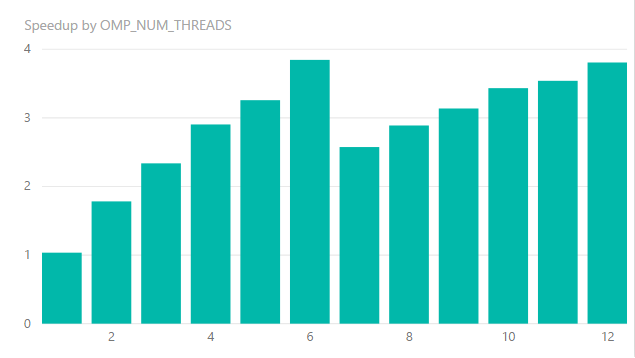
\includegraphics{pics/static.png}
\end{figure}

From 1 to 6 threads, the performance increases approximately linearly to 4x faster than single-threaded. However, with 7 threads,
performance is significantly reduced, and comes back to maximum at 12 threads.

With dynamic scheduling, the speedup is as follows:

\begin{figure}[h]
    \caption{Speedup with dynamic scheduling}
    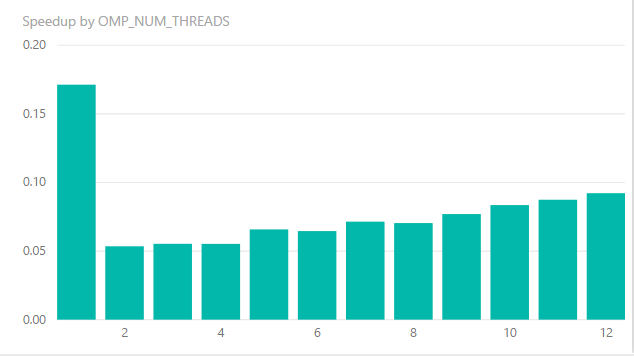
\includegraphics{pics/dynamic.png}
\end{figure}

Processing performance is highest when only 1 thread is used, but still significantly slower than normal CPU implementation.
With 2 threads, the program is 20x slower (0.05x speedup) compared to normal CPU implementation, and only slightly recovers
when the number of threads is increased to 12.

%%%%%%%%%%%%%%%%%%%%%%%%%%%%%%%%%%%%%%%%%%%%%%%%%%

\end{document}